\documentclass{article}

\usepackage{josuamathheader}
\newcommand{\rot}{\operatorname{rot}}
\renewcommand{\div}{\operatorname{div}}
\begin{document}
    \section*{Titel}
    \subsection{Maxwellgleichungen}
    Verbindung zwischen Feldern $\vec{E}, \vec{B}, \vec{D}, \vec{H}$ und den Ladungen $\rho, \vec{j}$.
    \begin{enumerate}
        \item \begin{align*}
            \div \vec{E} &= \nabla \cdot \vec{E} = \partial_i E^i = 4\pi \rho\\
            \int_V \intd^3 r \div \vec{E} &\stackrel{\text{Gauß}}{=} \int_{\partial V} \intd \vec{S} \cdot \vec{E} = \underset{\text{el. Fluss}}{\Psi} = \int_V \intd^3
        \end{align*}
        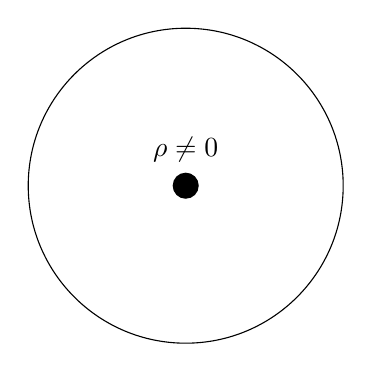
\begin{tikzpicture}
            \draw (0,0) circle (2cm);
            \node[fill = black, shape=circle, label=$\rho \neq 0$] (q) at (0,0) {}; 
        \end{tikzpicture}
        \item 
        \begin{align*}
            \div \vec{B} &= \nabla \times \vec{B} = \partial_i B^i = 0
        \end{align*}
        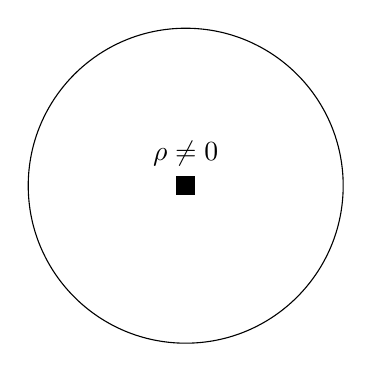
\begin{tikzpicture}
            \draw (0,0) circle (2cm);
            \node[fill = black, label=$\rho \neq 0$] (q) at (0,0) {};
        \end{tikzpicture}
        $\intd^3 r \div \vec{B} = \int_{ \partial V} \intd \vec{S} \cdot \vec{B} = \underset{\Phi}{\text{mag. Fluß}} = 0$
        Es gibt keine magnetische Ladung (elektromagnetische Dualität)
        \item $\rot \vec{E} = \nabla \times \vec E = -\partial_{ct} \vec B$. Faraday-Induktionsgesetz
        $\int_S \intd S \rot \vec E \stackrel{\text{Stokes}}{=} \int_{\partial S} \intd \vec r \cdot \vec E = \underset{U}{\text{Spannung}} = -\underbrace{\frac{\int d}{\intd (ct)}}{\frac{1}{c}\frac{\intd}{\intd t}} \int \intd \vec S \cdot \vec B = -\frac{\int d}{\intd (ct)} \Phi$
        \item 
        \[\rot \vec B = \nabla \times \vec B = \partial_{ct} \vec E + \frac{4\pi}{c} \vec j \hspace*{4cm} \text{Ampere-Gesetz.}
        \] 
        \[
            \int_S \intd \vec S\cdot \vec B \stackrel{\text{Stokes}}{=} \int_{\partial S} \intd \vec r \cdot \vec B = \frac{\intd}{\intd (ct)} \int_S \underbrace{\intd \vec S \cdot \vec E}_{=\Psi} + \frac{4\pi}{c}\underbrace{\int \intd \vec S \cdot \vec j}_{= I \text{ Strom}}
        \]
        zylindrische Symmetrie:
        \[
            \int_{\partial S} \intd \vec r \cdot \vec B = 4\pi r \left|\vec B(r)\right| = \frac{4\pi}{c} I \to \left|\vec B\right| \sim \frac{1}{r} 
        \]
    \end{enumerate}
\subsection*{Eigenschaften der Maxwell-Gleichungen}
\begin{itemize}
    \item lineare ($\to$ Superposition)
    \item partielle (Ableitungen in $x^i$ und $ct$ $\to \nabla, \partial_{ct}$)
    \item hyperbolische Differenzialgleichungen
    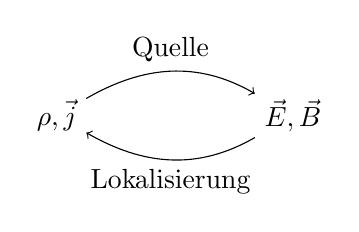
\begin{tikzpicture}
        \node (q) at (0,0) {$\rho, \vec j$};
        \node (E) at (3,0) {$\vec E, \vec B$};
        \draw[->] (q) to[out = 30, in=150] node[above] {Quelle} (E);
        \draw[->] (E) to[out = -150, in=-30] node[below] {Lokalisierung} (q);
    \end{tikzpicture}
    \item Inertialsystem
    \item Überbestimmtheit?
\end{itemize}
\subsection*{Erhaltung der elektrischen Ladung}
\begin{align*}
    \div \vec E &= 4\pi \rho &&| \partial_{ct}
    \rot \vec B &= \partial_{ct} \vec E + \frac{4\pi}{c} \vec{j} &&| \div
    \div \rot \vec B = 0 &= \partial_{ct} \div \vec E + \frac{4\pi}{c} \div \vec j\\
    &= 4\pi \partial_{ct} \rho + \frac{4\pi}{c} \div \vec j
\end{align*}
Daraus folgt die Kontinuitätsgleichung
\[
    \partial_{t} \rho + \div j = 0.  
\]
Es gilt
\[
    \frac{\intd}{\intd t} \int_V \intd^3 r \rho = \frac{\intd}{\intd t} q = - \int_V \intd^3 r \div \vec j \underset{\text{Gauß}}{=} -\int_{\partial V} \intd \vec S \cdot \vec j
\]
Elektrodynamik ist eien Kontinuumstheorie. Ladung ist eine Art \glqq Fluid \grqq.
\subsection*{Elektromagnetische Dualität}
$\rho = 0, \vec j = 0$.
\begin{enumerate}
    \item $\div \vec E = 0$
    \item $\div \vec B = 0$
    \item $\rot \vec E = -\partial_{ct} \vec B$
    \item $\rot \vec B = \partial_{ct} \vec E$.
\end{enumerate}
Vertauschung $\vec E \to \vec B,\quad \vec B \to -\vec E$ (Dualität).\\
Wieso gibt es eigentlich keine magnetische Ladung?
\begin{enumerate}
    \item $\div \vec E = 4\pi \rho$
    \item $\div \vec B = 4\pi \rho_m$
    \item $\rot \vec E = -\partial_{ct} \vec B + \frac{4\pi}{c}\vec{j}_m$
    \item $\rot \vec B = +\partial_{ct} \vec E + \frac{4\pi}{c} \vec j$
\end{enumerate}
Daraus würde folgen $\partial_t \rho_m + \div \vec j_m = 0$, analog zu $\partial_t \rho + \div \vec j = 0$.
\end{document}